\section{Tomografiakuvan muodostus}
Gammakameran kollimaattorin voidaan olettaa havaitsevan ainoastaan yhdestä suunnasta saapuvaa säteilyä. Tällöin gammakameran perspektiivistä havaitaan ikään kuin kaksiulotteinen varjo radioaktiivisen merkkiaineen kolmiulotteisesta jakaumasta. Keräämällä näitä projektioiksi kutsuttuja varjoja useasta suunnasta, voidaan matemaattisin menetelmin määrittää radioaktiivisen merkkiaineen jakauma.

Projektioiden matematiikka esitetään kahdessa ulottuvuudessa (jolloin projektiot ovat yksiulotteisia) ymmärrettävyyden vuoksi. Yleistys kolmeen ulottuvuuteen ja kaksiulotteiseen projektioon on suhteellisen suoraviivainen.

\begin{figure}[H]
    \centering
    \captionsetup{width=.9\textwidth}
    \begin{tikzpicture}
    \draw[->, thick] (-3,0)--(3,0) node[right]{$x$};
    \draw[->, thick] (0,-3)--(0,3) node[above]{$y$};


    \begin{scope}[shift={(0, 0)}, rotate=30]
        \begin{scope}[shift={(0, 5)}, rotate=180] % Detektori
            \draw[->, thick] (3.5, -1.3) -- (-3.5, -1.3) node[right]{$s$}; % s-akseli
            \draw[domain=-1.5:1.5, smooth, variable=\s, red] plot ({\s}, {-2.3-cos(2 * pi / 3 * \s r)}) node[above left]{$g(s, \theta)$};

            % Kollimaattori
            \foreach \x in {-3.5, -3.2, ..., 3.5}
            \fill (\x,0) rectangle (\x + 0.1,1);
    
            % Tuikeaine
            \draw (-3.5, 0) rectangle (3.5, -1);
            \fill[pattern=north east lines] (-3.5, 0) rectangle (3.5, -1);
        \end{scope}
        % Aktiivisuusjakauma
        \fill[pattern=dots, pattern color=blue] (0,0) circle (1.5) node[below left]{$f(x, y)$};

        % Suora
        \draw[dashed, red] (0.9, -3) -- (0.9, 5);
    \end{scope}
\end{tikzpicture}
    \caption{Aktiivisuusjakauma $f$ $xy$-tasossa (siniset pisteet), gammakamera (mustat palkit ja väritetty alue) ja projektio $g(s, \theta)$, jossa $\theta$ on $s$- ja $x$-akseleiden välinen kulma. Yhteen projektion pisteeseen vaikuttava aktiivisuusjakauman osa on piirretty punaisella katkoviivalla. Kuva on muokattu lähteestä \cite{bruyant_analytic_2002}.}
    \label{fig:projektio}
\end{figure}

Tarkastellaan $xy$-tason jatkuvaa aktiivisuusjakaumaa $f\colon\RR^{2}\to\RR$. Olkoon $\theta$ gammakameran tangentin ja positiivisen $x$-akselin välinen kulma kuten \hyperref[fig:projektio]{kuvassa \ref*{fig:projektio}}. Merkitään projektiota $g(s, \theta)$, jossa $s$ on gammakameran tangentin suuntainen koordinaattiakseli.

Kulmalla $\theta$ ja pisteessä $s$ gammakamera havaitsee säteilyä $xy$-tason suoralta $\Omega$, jonka määrittää
\begin{equation*}
    \Omega=\left\{ (x, y) \mid x\cos(\theta)+y\cos(\theta)=s \right\}.
\end{equation*}
Projektio, eli suoralta $\Omega$ havaittu säteily voidaan esittää siten Radon-muunnokseksi kutsuttuna polkuintegraalina\cite{radon_determination_1986, bruyant_analytic_2002}
\begin{equation}\label{eqn:radon-muunnos}
    g(s, \theta)=\int_{\Omega}f(x, y).
\end{equation}

Tietokoneella voidaan kuitenkin käsitellä ainoastaan äärellistä määrää mitattuja projektioita. Toisin sanoen muuttujat $s$ ja $\theta$ ovat diskreettejä, jonka vuoksi on luontevaa käsitellä myös muuttujia $x$ ja $y$ diskreetteinä jakamalla kuva-alue pikseleihin, joissa aktiivisuusjakaumat ovat vakioita.

\begin{figure}[H]
    \centering
    \captionsetup{width=.9\textwidth}
    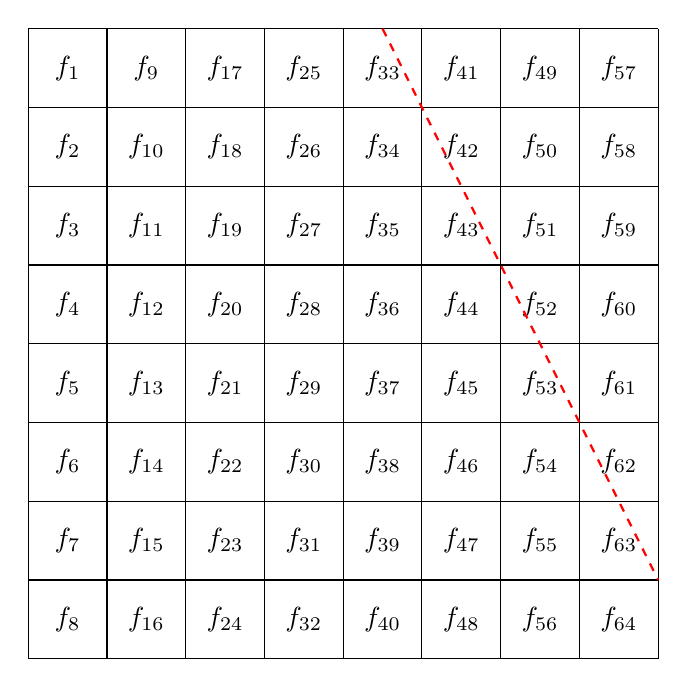
\begin{tikzpicture}
    % Vaakasuorat viivat
    \foreach \i in {0,1,...,8} {
        \draw (0, \i) -- (8, \i);
    }   

    % Pystysuorat viivat
    \foreach \j in {0,1,...,8} {
        \draw (\j, 0) -- (\j, 8);
    }

    % Pikselien indeksit
    \foreach \i in {0,1,...,7} {
        \foreach \j in {0,1,...,7} {
            \node at (\j+0.5, \i+0.5) {$f_{\the\numexpr \j*8 + (8 - \i) \relax}$};
        }
    }

    % Projektion suora
    \draw[thick, dashed, red] (4.5, 8) -- (8, 1);
\end{tikzpicture}
    \caption{Kuva-alue (ruudukko), kuva-alueen pikselit $f_i$, $i=1,\ldots,64$ ja projektion suora piirrettynä punaisella katkoviivalla.}
    \label{fig:diskreetti-projektio}
\end{figure}

Kun kuva-alue jaetaan pikseleihin, joihin viitataan indekseillä $i=1,\ldots, n$, yhtälön (\ref{eqn:radon-muunnos}) integraali voidaan jakaa pikselikohtaisesti osiin
\begin{alignat*}{2}
    g(s, \theta)
    &=\sum_{i=1}^{n}\int_{\Omega}f(x, y)\chi_{i}.
\end{alignat*}
Funktio $\chi_i$ on indikaattorifunktio, joka saa arvon 1 pikselin $i$ sisällä ja arvon 0 kaikkialla muualla.

Oletetaan kuva-alueen aktiivisuusjakauma paloittain vakioksi pikselikohtaisesti. Tällöin voidaan merkitä
\begin{equation*}
    f(x, y)\chi_{i}=f_i.
\end{equation*}
Yhtälön (\ref{eqn:radon-muunnos}) integraali palautuu summaksi
\begin{equation}\label{eqn:diskreetti-radon-muunnos}
    g(s, \theta)=\sum_{j=1}^{n}a_{j}f_{j},
\end{equation}
jossa $a_i$ on suoran $\Omega$ kulkema matka pikselissä $i$. 

\hyperref[fig:diskreetti-projektio]{Kuvassa \ref*{fig:diskreetti-projektio}} projektion suora kulkee kuva-alueen pikseleiden 33, 42, 43, 52, 53, 62 ja 63 lävitse. Suoran kulkema matka on jokaisessa edellä mainitusta pikselissä $\frac{\sqrt{5}}{2}$.

Toisaalta kertoimet $a_i$ määräävät parametrit $s$ ja $\theta$ täysin. Merkitään tästä johtuen yhtä projektiota, eli havaintoa, $g_i$ ja vastaavia kertoimia $a_{ij}$. Havainnot
\begin{equation*}
    \begin{cases}
        g_1&=\sum_{j=1}^{n}a_{1j}f_{j}\\
        &\vdots\\
        g_m&=\sum_{j=1}^{n}a_{mj}f_{j}
    \end{cases}
\end{equation*}
voidaan kerätä matriisiyhtälöön $g=Af$, jossa $g=\left( g_1, \ldots, g_m \right)^{T}$, $f=\left( f_1, \ldots, f_m \right)^{T}$ ja matriisi $A$,
\begin{equation*}
    A=
    \begin{pmatrix}
        a_{11} & a_{12} & \cdots & a_{1n} \\
        a_{21} & a_{22} & \cdots & a_{2n} \\
        \vdots & \vdots & \ddots & \vdots \\
        a_{m1} & a_{m2} & \cdots & a_{mn}
    \end{pmatrix},
\end{equation*}
on projektio-operaattori.

\subsection{Analyyttiset menetelmät}
\textcolor{red}{FBP}

\subsection{Iteratiiviset menetelmät}
\textcolor{red}{MLEM, OSEM}

\subsection{Virhelähteet kuvanmuodostuksessa}
\subsection{OMEGA}